%%%%%%%%%%%%%%%%%%%%%%%%%%%%%%%%%%%
%This is the LaTeX ARTICLE template for RSC journals
%Copyright The Royal Society of Chemistry 2016
%%%%%%%%%%%%%%%%%%%%%%%%%%%%%%%%%%%

\documentclass[twoside,twocolumn,9pt]{article}
\usepackage{extsizes}
\usepackage[super,sort&compress,comma]{natbib} 
\usepackage[version=3]{mhchem}
\usepackage[left=1.5cm, right=1.5cm, top=1.785cm, bottom=2.0cm]{geometry}
\usepackage{balance}
\usepackage{mathptmx}
\usepackage{sectsty}
\usepackage{graphicx} 
\usepackage{lastpage}
\usepackage[format=plain,justification=justified,singlelinecheck=false,font={stretch=1.125,small,sf},labelfont=bf,labelsep=space]{caption}
\usepackage{float}
\usepackage{fancyhdr}
\usepackage{fnpos}
\usepackage[english]{babel}
\addto{\captionsenglish}{%
  \renewcommand{\refname}{Notes and references}
}
\usepackage{array}
\usepackage{droidsans}
\usepackage{charter}
\usepackage[T1]{fontenc}
\usepackage[usenames,dvipsnames]{xcolor}
\usepackage{setspace}
\usepackage[compact]{titlesec}
\usepackage{hyperref}
%%%Please don't disable any packages in the preamble, as this may cause the template to display incorrectly.%%%


\usepackage{balance}
\usepackage{times,mathptmx}
\usepackage{sectsty}
\usepackage{graphicx} 
\usepackage{lastpage}
\usepackage[format=plain,justification=justified,singlelinecheck=false,font={stretch=1.125,small,sf},labelfont=bf,labelsep=space]{caption}
\usepackage{float}
\usepackage{fancyhdr}
\usepackage{fnpos}
\usepackage[english]{babel}
\addto{\captionsenglish}{%
  \renewcommand{\refname}{Notes and references}
}
\usepackage{array}
\usepackage{droidsans}
\usepackage{charter}
\usepackage[T1]{fontenc}
\usepackage[usenames,dvipsnames]{xcolor}
\usepackage{setspace}
\usepackage[compact]{titlesec}
\usepackage{hyperref}

\usepackage{abstract}
\usepackage{graphicx}
\usepackage{gensymb}
\usepackage{caption}
\usepackage{amsmath}
\usepackage{amsthm}
\usepackage{amsfonts}
%\usepackage{float}
\usepackage{sidecap}
\usepackage{mathtools}
\usepackage{adjustbox}
\usepackage{ upgreek }




\usepackage{epstopdf}%This line makes .eps figures into .pdf - please comment out if not required.

\definecolor{cream}{RGB}{222,217,201}

\begin{document}

\pagestyle{fancy}
\thispagestyle{plain}
\fancypagestyle{plain}{
%%%HEADER%%%
\renewcommand{\headrulewidth}{0pt}
}
%%%END OF HEADER%%%

%%%PAGE SETUP - Please do not change any commands within this section%%%
\makeFNbottom
\makeatletter
\renewcommand\LARGE{\@setfontsize\LARGE{15pt}{17}}
\renewcommand\Large{\@setfontsize\Large{12pt}{14}}
\renewcommand\large{\@setfontsize\large{10pt}{12}}
\renewcommand\footnotesize{\@setfontsize\footnotesize{7pt}{10}}
\makeatother

\renewcommand{\thefootnote}{\fnsymbol{footnote}}
\renewcommand\footnoterule{\vspace*{1pt}% 
\color{cream}\hrule width 3.5in height 0.4pt \color{black}\vspace*{5pt}} 
\setcounter{secnumdepth}{5}

\makeatletter 
\renewcommand\@biblabel[1]{#1}            
\renewcommand\@makefntext[1]% 
{\noindent\makebox[0pt][r]{\@thefnmark\,}#1}
\makeatother 
\renewcommand{\figurename}{\small{Fig.}~}
\sectionfont{\sffamily\Large}
\subsectionfont{\normalsize}
\subsubsectionfont{\bf}
\setstretch{1.125} %In particular, please do not alter this line.
\setlength{\skip\footins}{0.8cm}
\setlength{\footnotesep}{0.25cm}
\setlength{\jot}{10pt}
\titlespacing*{\section}{0pt}{4pt}{4pt}
\titlespacing*{\subsection}{0pt}{15pt}{1pt}
%%%END OF PAGE SETUP%%%

%%%FOOTER%%%
\fancyfoot{}
\fancyfoot[LO,RE]{\vspace{-7.1pt}\includegraphics[height=9pt]{head_foot/LF}}
\fancyfoot[CO]{\vspace{-7.1pt}\hspace{13.2cm}\includegraphics{head_foot/RF}}
\fancyfoot[CE]{\vspace{-7.2pt}\hspace{-14.2cm}\includegraphics{head_foot/RF}}
\fancyfoot[RO]{\footnotesize{\sffamily{1--\pageref{LastPage} ~\textbar  \hspace{2pt}\thepage}}}
\fancyfoot[LE]{\footnotesize{\sffamily{\thepage~\textbar\hspace{3.45cm} 1--\pageref{LastPage}}}}
\fancyhead{}
\renewcommand{\headrulewidth}{0pt} 
\renewcommand{\footrulewidth}{0pt}
\setlength{\arrayrulewidth}{1pt}
\setlength{\columnsep}{6.5mm}
\setlength\bibsep{1pt}
%%%END OF FOOTER%%%

%%%FIGURE SETUP - please do not change any commands within this section%%%
\makeatletter 
\newlength{\figrulesep} 
\setlength{\figrulesep}{0.5\textfloatsep} 

\newcommand{\topfigrule}{\vspace*{-1pt}% 
\noindent{\color{cream}\rule[-\figrulesep]{\columnwidth}{1.5pt}} }

\newcommand{\botfigrule}{\vspace*{-2pt}% 
\noindent{\color{cream}\rule[\figrulesep]{\columnwidth}{1.5pt}} }

\newcommand{\dblfigrule}{\vspace*{-1pt}% 
\noindent{\color{cream}\rule[-\figrulesep]{\textwidth}{1.5pt}} }

\makeatother
%%%END OF FIGURE SETUP%%%

%%%TITLE, AUTHORS AND ABSTRACT%%%
\twocolumn[
  \begin{@twocolumnfalse}
{\includegraphics[height=30pt]{head_foot/journal_name}\hfill\raisebox{0pt}[0pt][0pt]{\includegraphics[height=55pt]{head_foot/RSC_LOGO_CMYK}}\\[1ex]
\includegraphics[width=18.5cm]{head_foot/header_bar}}\par
\vspace{1em}
\sffamily
\begin{tabular}{m{4.5cm} p{13.5cm} }

\includegraphics{head_foot/DOI} & \noindent\LARGE{\textbf{A High-Throughput Computational Dataset of Halide Perovskite Alloys$^\dag$}} \\%Article title goes here instead of the text "This is the title"
\vspace{0.3cm} & \vspace{0.3cm} \\

 & \noindent\large{Jiaqi Yang,\textit{$^{a}$} Panayotis Manganaris\textit{$^{a}$} and Arun Mannodi-Kanakkithodi\textit{$^{a}$}} \\%Author names go here instead of "Full name", etc.

\includegraphics{head_foot/dates} & \noindent\normalsize{The great tunability of the properties of halide perovskites presents new opportunities for optoelectronic applications as well as significant challenges associated with exploring combinatorial chemical spaces. In this work, we develop a framework powered by high-throughput computations and machine learning for the design and prediction of mixed cation halide perovskite alloys. In a chemical space of ABX$_{3}$ perovskites with a selected set of options for A, B, and X atoms, pseudo-cubic structures of compounds with B-site mixing are simulated using density functional theory (DFT) and several properties are computed, including stability, lattice constant, band gap, vacancy formation energy, refractive index, and optical absorption spectrum, using both semi-local and hybrid functionals. Neural networks (NN) are used to train predictive models for every property using tabulated elemental properties of A, B, and X site atoms as descriptors. Starting from the DFT dataset of 229 points, we use the trained NN models to predict the structural, energetic, electronic and optical properties of a complete dataset of 17,955 compounds, and perform high-throughput screening in terms of stability, band gap and defect tolerance, to obtain 574 promising compounds that are ranked as potential absorbers according to their photovoltaic figure of merit. Compositional trends in the screened set of attractive mixed cation halide perovskites are revealed and additional computations are performed on selected compounds. The data-driven design framework developed here is promising for designing novel mixed compositions and can be extended to a wider perovskite chemical space in terms of A, B, and X atoms, different kinds of mixing at the A, B, or X sites, non-cubic phases, and other properties of interest.} 

\end{tabular}

 \end{@twocolumnfalse} \vspace{0.6cm}

  ]
%%%END OF TITLE, AUTHORS AND ABSTRACT%%%

%%%FONT SETUP - please do not change any commands within this section
\renewcommand*\rmdefault{bch}\normalfont\upshape
\rmfamily
\section*{}
\vspace{-1cm}


%%%FOOTNOTES%%%

\footnotetext{\textit{$^{a}$~School of Materials Engineering, Purdue University, West Lafayette, IN 47907, USA; E-mail: amannodi@purdue.edu }}

\footnotetext{\dag~Electronic Supplementary Information (ESI) available: [details of any supplementary information available should be included here]. See DOI: 00.0000/00000000.}


%%%END OF FOOTNOTES%%%

%%%MAIN TEXT%%%%


\section*{Introduction}

... \\

% \begin{figure*}[h]
% \centering
% 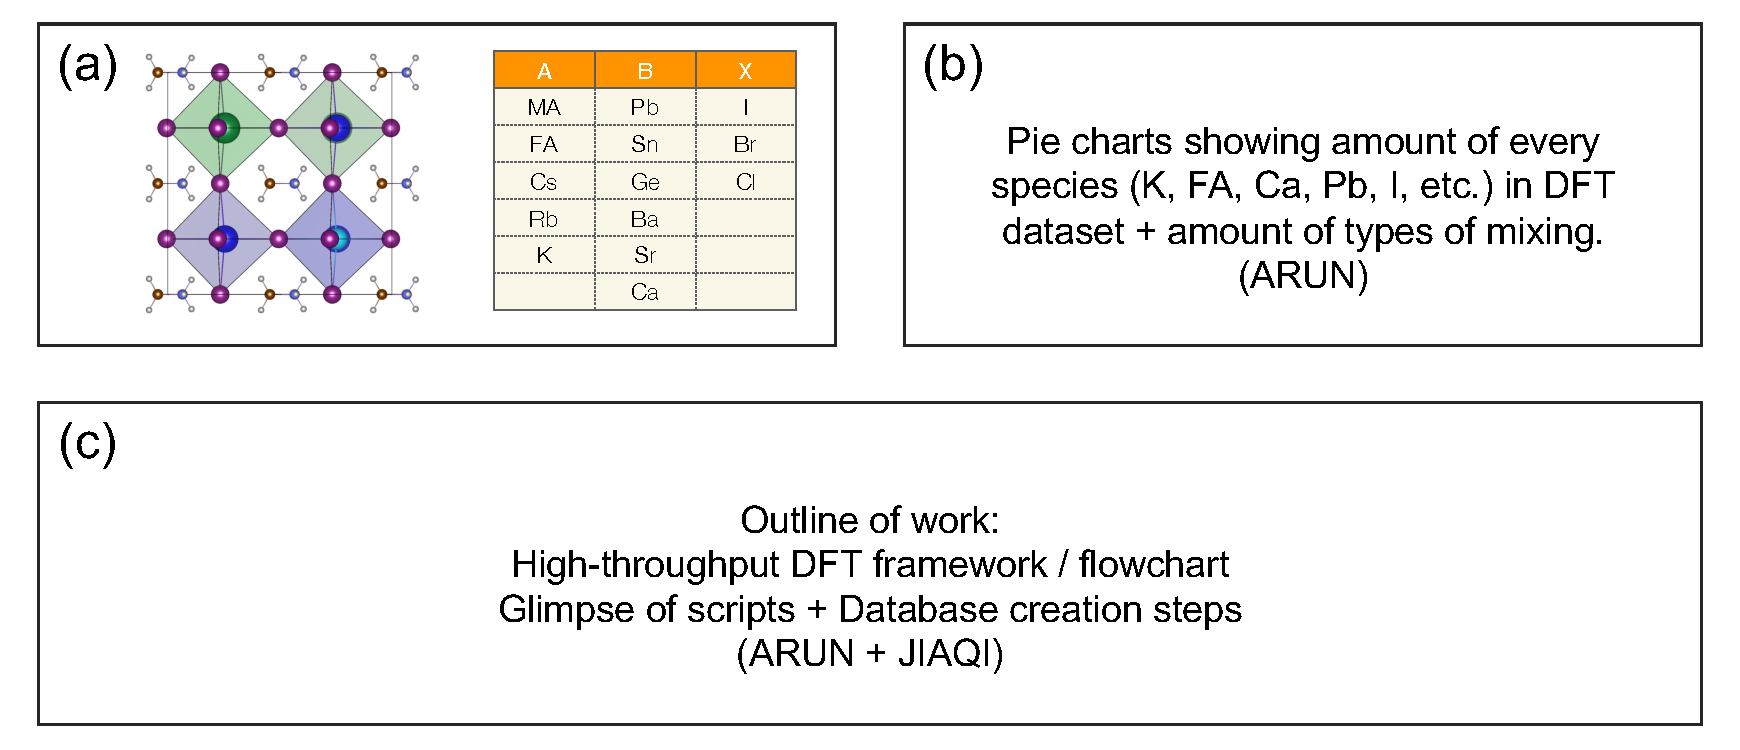
\includegraphics[width=0.80\linewidth]{Figure1.pdf}
% \caption{\label{Fig:outline} 
% (a) DFT properties computed for 229 perovskite compounds at the PBE and HSE06 levels of theory. (b) Typical neural network architecture used to train predtictive models from DFT data. (c) Screening performed on ML predicted dataset of 17,955 perovskite compounds in terms of their stability, band gaps and defect tolerance.}
% \end{figure*}

\newpage



\section*{Methodology}

\subsection*{DFT Details}

% \begin{equation}\label{eqn-0}
% \begin{multlined}
% FOM = \sum_{\lambda_i} \alpha(\lambda_i) * I_s(\lambda_i) * (\lambda_{i+1} - \lambda_i) / \sum_{\lambda_i} I_s(\lambda_i) * (\lambda_{i+1} - \lambda_i)
% \end{multlined}
% \end{equation}

\subsection*{Accessing and Analyzing DFT Data}

\subsection*{Data Visualization Methods}

\newpage




\section*{Results and discussion}

\subsection*{Visualization of DFT Data}

... \\

% \begin{table}
% \centering
%   \caption{\ NN model training and test prediction RMSEs for every property.}
%   \label{table:rmse}
%   \begin{tabular}{ccc}
%     \hline
%   &   &   \\
% \textbf{Property}  &  \textbf{Training Set RMSE}  &  \textbf{Test Set RMSE} \\
%   &   &   \\
% \hline
%   &   &   \\
%       PBE Lattice Constant  & 0.09 \AA  & 0.10 \AA  \\
%       HSE Lattice Constant  & 0.06 \AA  & 0.06 \AA  \\
%       $\Delta$H$_{decomp}$ (PBE) & 0.05 eV  & 0.11 eV  \\
%       $\Delta$H$_{decomp}$ (HSE)  & 0.05 eV  & 0.09 eV  \\
%       E$_{gap}$$^{PBE}$  & 0.20 eV  & 0.22 eV  \\
%       E$_{gap}$$^{HSE}$  & 0.19 eV  & 0.24 eV  \\
%       Refractive Index  & 0.04  & 0.05  \\
%       PV FOM (log$_{10}$)  & 0.14  & 0.18  \\
%       X-rich D.F.E.  & 0.12 eV  & 0.23 eV  \\
%       X-rich E$_{F}$  & 0.06 eV  & 0.19 eV  \\
%       Medium-X D.F.E.  & 0.18 eV  & 0.29 eV  \\
%       Medium-X E$_{F}$  & 0.11 eV  & 0.30 eV  \\
%       B-rich D.F.E.  & 0.11 eV  & 0.30 eV  \\
%       B-rich E$_{F}$  & 0.11 eV  & 0.25 eV  \\
%       V$_{A}$ (0/-1) & 0.07 eV  & 0.11 eV  \\
%       V$_{X}$ (+1/0)  & 0.19 eV  & 0.22 eV  \\
%   &   &   \\
%     \hline
%   \end{tabular}
% \end{table}

\newpage



\section*{Perspective and Future Work}
    
... \\



\section*{Conclusions}

... \\


\section*{Conflicts of interest}
There are no conflicts to declare.

\section*{Acknowledgements}
Extensive discussions with and scientific feedback from UC San Diego researchers David Fenning and Rishi Kumar and Argonne National Lab scientist Maria Chan are acknowledged. This work was performed at Purdue University, under startup account F.10023800.05.002 from the Materials Engineering department. This research used resources of the National Energy Research Scientific Computing Center, the Laboratory Computing Resource Center at Argonne National Laboratory, and the RCAC clusters at Purdue.


\balance


\bibliography{rsc} %You need to replace "rsc" on this line with the name of your .bib file
\bibliographystyle{rsc} %the RSC's .bst file





\clearpage
\newpage
\setcounter{page}{1}

%\onecolumngrid

\setcounter{figure}{0}   
\setcounter{table}{0} 
\renewcommand{\thetable}{S\Roman{table}} 
\renewcommand\thefigure{S\arabic{figure}}
 
\begin{center}
\vspace*{0.5cm}
\Large
\textbf{Supplemental material to "A High-Throughput Computational Dataset of Halide Perovskite Alloys"\\}
\vspace{0.5cm}
\large
Jiaqi Yang,\textit{$^{a}$} Panayotis Manganaris\textit{$^{a}$} and Arun Mannodi-Kanakkithodi\textit{$^{a}$} \\
\vspace{0.3cm}

\normalsize
\textsuperscript{a}\textit{School of Materials Engineering, Purdue University, West Lafayette, Indiana 47907, USA} \\
\end{center}

\footnote{
\textsuperscript{a}amannodi@purdue.edu\hspace{0.3cm}}

\vspace{1cm}



% \begin{figure*}[h]
% \centering
% \includegraphics[width=\linewidth]{SI_figs/Table_elem_prop.pdf}
% \caption{\label{Fig:SI_elem_prop} 
% List of 15 elemental/molecular properties and tabulated values used for each A, B and X-site constituent in the halide perovskite chemical space.}
% \end{figure*}


% \begin{table*}[h]
% \centering
%   \caption{\ Calculated PV figures of merit (in log$_{10}$) for known semiconductors and some selected compounds from the current study.}
%   \label{table:SI_FOM}
%   \begin{tabular}{cc}
%     \hline
%   &   \\
% \textbf{Compound}  &  \textbf{log$_{10}$ (PV FOM)} \\
%   &   \\
% \hline
%   &   \\
% Si    &   5.64   \\
% SiC   &   3.76   \\
% GaAs   &   5.66   \\
% CdTe   &   5.46   \\
% CdSe   &   5.31   \\
% 	   &   \\
% CsCa$_{0.25}$Ba$_{0.125}$Ge$_{0.25}$Pb$_{0.375}$Cl$_{3}$   &   4.72   \\
% MACa$_{0.375}$Ge$_{0.5}$Pb$_{0.125}$Br$_{3}$   &   4.88   \\
% MACa$_{0.125}$Sr$_{0.125}$Ba$_{0.125}$Ge$_{0.125}$Pb$_{0.5}$I$_{3}$   &   5.07   \\
% CsCa$_{0.875}$Pb$_{0.125}$Br$_{3}$   &   3.84   \\
% FACa$_{0.125}$Sr$_{0.375}$Ba$_{0.125}$Sn$_{0.125}$Pb$_{0.25}$I$_{3}$   &   4.88   \\
%   &   \\
%     \hline
%   \end{tabular}
% \end{table*}

\end{document}
